\section{Abordagem proposta}
% Nessa seção devem ser apresentados os métodos utilizados no trabalho, ferramentas, dados e materiais.

Empresas que atuam em uma grande área do território nacional atendendo a um grande número de clientes podem ser ré de diversas ações judiciais iniciadas pelos consumidores que se sentiram lesados com os serviços prestados. Desse modo, essas numerosas ações judiciais podem ocorrer em diferentes locais ou comarcas, \enquote{\textit{território em que o juiz de primeiro grau irá exercer sua jurisdição e pode abranger um ou mais municípios}} \cite{cnj:comarca}, o que dificulta o acompanhamento dos processos forenses. Assim sendo, manter uma equipe jurídica do tamanho necessário para cuidar dessa volumosa soma de processos, manualmente, pode ser muito custoso para a empresa, sendo capaz de prejudicar a bem-estar financeiro e jurídico dela.

Diante desse cenário, surgiram empresas que ofertam \enquote{inteligência jurídica}, acompanhando os inúmeros processos jurídicos por meio da sua coleta, armazenando-os em um banco de dados. Esses dados processuais são disponibilizados pelos sistemas de justiça providenciados por meio das suas plataformas digitais como o Projudi do TJPE \cite{tjpe} e o e-SAJ CE \cite{esajce}. Essa coleta otimiza o trabalho das equipes jurídicas das empresas, no entanto, esses dados podem ser usados para fornecer muito mais informações para o setor jurídico da empresa e até contribuir para o seu \textit{business intelligence} (BI), revelando novas perspectivas que servirão de base para a tomada de decisão.

Mas no Brasil existem diversas plataformas digitais de justiça, em que cada uma disponibiliza os dados a sua maneira. Essa diferenciação na representação de um mesmo tipo de informação é uma problema quando se deseja usar técnicas de \textit{business intelligence} por meio de um \textit{data warehouse} (Seção \ref{subsec:datawarehouse}), pois sem um tratamento prévio, o agrupamento dos dados nessa situação não apresenta resultados satisfatórios. Então é necessário utilizar alguma estratégia para padronizar esses dados, sendo o ETL (Seção \ref{subsec:etl}) uma das técnicas mais utilizadas para tal.

\subsection{Processos}
\label{processos}

As elementos contidos no processo são imprescindíveis para a construção do \textit{data warehouse} focado na obtenção de conhecimento jurídico e na aplicação da jurimetria, isto é, a \enquote{\textit{é a estatística aplicada ao Direito}} \cite{newlawJurimetria}.

Os principais dados de um processo judicial são a sua Numeração Processual Única (NPU) ou somente número, as partes envolvidas e os andamentos ou movimentações.

A NPU é composta por vinte dígitos e foi instituído pelo Conselho Nacional de Justiça (CNJ) com o intuito de facilitar a consulta das informação referente a um processo, pois os números dos processos mudavam em cada instância ou recurso. A Numeração Processual Única vale para os tribunais de todo o país e apresentam a seguinte estrutura \enquote{NNNNNNN-DD.AAAA.J.TR.OOOO} no qual \cite{jusbrasilNPU}:

\begin{itemize}
    \item \textbf{NNNNNNN-DD}: representam o número sequencial do processo e seu dígito verificador \cite{TRF4NPU}.
    \item \textbf{AAAA}: diz respeito ao ano de avaliação do processo \cite{TRF4NPU}.
    \item \textbf{J}: informa qual o órgão ou segmento do Poder Judiciário que o processo pertence \cite{TRF4NPU}.
    \item \textbf{TR}: indica o tribunal do respectivo segmento ou circunscrição judiciária \cite{TRF4NPU}.
    \item \textbf{OOOO}: remete à unidade de origem do processo \cite{TRF4NPU}.
\end{itemize}

As partes do processo são compostas pelo autor, que desempenha o papel de polo ativo do processo, ou seja, aquele que recorre a tutela jurídica do estado, tomando a posição ativa, e pelo réu, que realiza o papel do polo passivo, estando sujeito a ação processual iniciada pelo autor.

Por fim, as movimentações de um processo são um conjunto de informações que comunicam a evolução processual ao longo da tramitação. Elas podem conter os mais diferentes tipos de conhecimentos a respeito do processo, como os informes sobre o dia de uma audiência, notificação de emissão de intimação ou até mesmo a notícia da sentença do juiz.

\subsection{ETL para Jurimetria}
\label{jurimetria}

A técnica de ETL usada neste trabalho segue o modelo de filas FIFO (\textit{First In, First Out} - primeiro a entrar, primeiro a sair) (Figura \ref{fig:stepsFlow}). Cada nó dessa fila é uma estrutura que recebe o nome de \textit{step}.

\begin{figure}[ht]
\centering
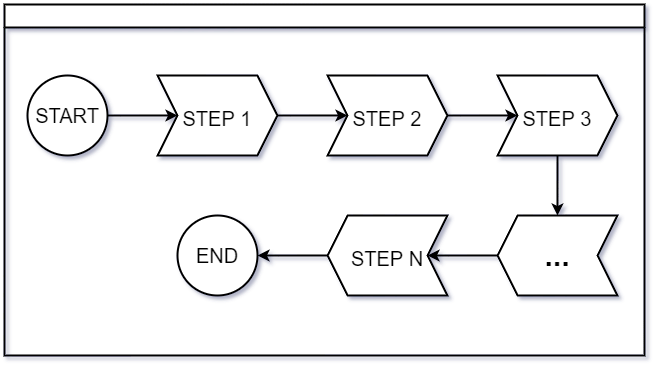
\includegraphics[width=1\textwidth]{imagens/steps-flow.png}
\caption{Exemplo do fluxo dos \textit{steps}.}
\label{fig:stepsFlow}
\end{figure}

O \textit{step} é um conjunto de operações que serão aplicada ao processo para realizar um objetivo bem definido. No projeto, ele é codificado como uma classe Python (Seção \ref{subsec:python}) com um método obrigatório chamado \textit{transform}. O \textit{transform} é a função que receberá o processo e aplicará as transformações e inferências necessárias para atingir o seu objetivo.

\begin{figure}[ht]
\centering
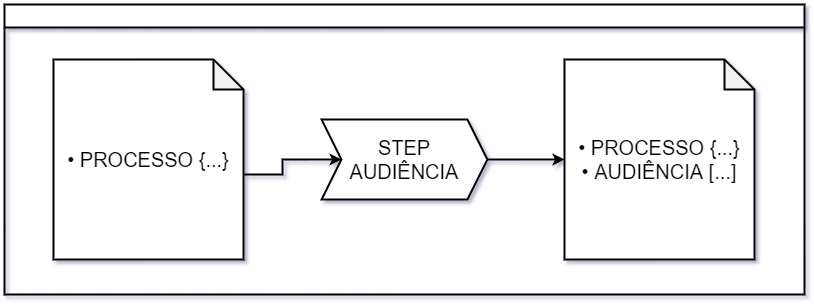
\includegraphics[width=1\textwidth]{imagens/processo-in-step.png}
\caption{Exemplo de \textit{step} enriquecendo o documento com novas informações.}
\label{fig:processoInStep}
\end{figure}

Os processos são extraídos dos vários sistemas jurídicos pela equipe de extração e armazenados como documentos em um banco de dados MongoDB (Seção \ref{subsec:mongo}). Esses documentos serão usados no processamento do ETL que preparará os dados para serem inseridos no \textit{data warehouse}. No ETL, os documentos são lidos do MongoDB e estruturados como um dicionário do Python (Figura ).

% TODO inserir imagem do processo como um dicionário python

\subsubsection{Steps}
\label{steps}

Para esse trabalho, não serão abordados todos os \textit{steps} que são efetivamente realizados na empresa, mas somente um recorte de alguns dos mais importantes. Com exceção do primeiro \textit{step}, que trata da normalização dos dados, cada um dos demais \textit{steps} são responsáveis pela criação de uma nova tabela no banco de dados final.

% TODO Escreve sobre os steps.
O primeiro \textit{step} é chamado de...